\chapter{Methods}
%may want to rewrite first paragraph, too much I
I want the framework and methods used to be easy to use and understand, so that it can be discussed among clinicians and other people who don't have a statistics or mathematics background. On the same token, I want the methods and theory to be sound from a statistical point of view. There are many different theories and implementations to choose from for the three topics covered in this thesis. I aim to pick the ones that optimize ease of understanding and power of results, with the motivating example being cancer survival data. Throughout this section, decisions must be made as to what methods and analyses to use. Whenever a decision is made, I explain why it was chosen as well as alternative methods that could also be used. It is my hope that I will provide enough clarity and detail so that the interested reader can intelligently apply these methods to their own data, even if the choice of methods is different than this thesis.
\section{Multiple Imputation}
\label{sec:MI}
It should be clear that multiple imputation is the preferred method to deal with missing data, so our first decision comes as to what paradigm to impute under. As long as valid imputations are produced, the choice of method to generate the imputations does not matter. However, since the base of our analysis starts with imputation, we need to make sure that we pick a good method. Everything that follows in the analysis is dependent on our imputed data, so it is necessarily the case that poor imputations will lead to poor results be it bias, high variability, or loss in statistical power.
\subsection{Selecting the MI scheme}

There are two main divisions in modern multiple imputation:  joint modelling and full conditional specification. Both have their own advantages and flaws. I will describe both, and then explain why full conditional specification is better suited for cancer research.

Before we get in to the imputation models, we need to have a firm understanding of missing data concepts. They take up quite a bit of space to explain, but they are fundamental concepts. I suggest that everyone reads appendix \ref{app:apdx} (even if you are familiar with MI), so that the concepts and symbols that will be used in this paper are understood and standardized. 

The first main imputation strategy is called Joint Modelling (JM). In JM, we assume that the missing data mechanism is ignorable and that the data can be described by a multivariate distribution specified by the user on the rows (missing data pattern) of the data. Then, we run a sampler that draws imputations from the specified model, and updates model parameters. Since the true model parameters are unknown, they need to be estimated. This is often done by a data augmentation algorithm \cite{VanBuuren2012}.  A pseudocode example will help better clarify the steps, as can be seen in figure \ref{fig:jmexample}, where the assumed model is a multivariate normal.
\begin{figure}[h!]
  \centering
    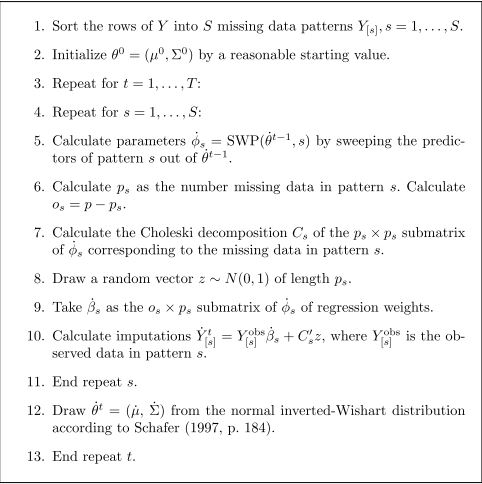
\includegraphics[width=0.8\textwidth]{jm_algo}
  \caption{Normal JM imputation pseudocode}
\label{fig:jmexample}
\medskip
\small
Taken from van Buuren's book �Flexible imputation of missing data� \cite{VanBuuren2012}
\end{figure}

There has been extensive programming and research on using the normal model for this, and research shows that it even performs well under situations where the data has strong non-normality \cite{Demirtas2008}. Not much research has been done on models outside of the normal. 

This is just one implementation of a JM approach. Another, like that used in the Amelia package, uses an EM algorithm to draw from the missing data's posterior assuming a normal likelihood and user specified priors \cite{Honaker2015}.  Other distributions can be used, but the user will have to specify it, derive any relevant distributions, program it, and research to see if the method provides optimal properties, such as proper coverage and correct estimation of the parameters of interest.

An obvious issue with JM arises when the data is categorical (either alone or mixed in with continuous). There has been much debate in the literature about how to handle this situation. Some authors argue that you should just impute under a continuous distribution and round imputations to the nearest class number, and others suggest using distributions that are more suited for categorical data \cite{VanBuuren2012}. However, no consensus has been reached on the best method. 

\begin{comment}
A few of the most used R packages for joint modelling imputation include Amelia \cite{Honaker2015}, norm \cite{norm2015} and cat \cite{cat2015}.
\end{comment}
It is my opinion that unless the user is very confident in the multivariate joint distribution, that JM should not be used. In the cancer example, there are many categorical variables and strictly positive variables to impute, so JM seems inappropriate.

The other MI strategy is called fully conditional specification (FCS). In this paradigm, missing data is assumed to be MAR (although it can work on MNAR with more assumptions), and is imputed on a variable by variable case on the columns/covariates based off of user specified imputation models. Whereas JM imputes on the rows, FCS imputes on the columns. Imputations are drawn from the missing data's posterior predictive distribution. This theory goes by many names, including partially compatible MCMC, iterated univariate imputation, and chained equations \cite{VanBuuren2012}. In the JM setting, the user must give one $k$ dimensional model, however in the FCS setting, the user must give k one dimensional models. The goal of FCS methods are to sample from
%I take out the X's here to keep consistent with the apdx
$$P(Y,R|\theta)$$
By sampling from the full conditionals
$$P(Y_j|Y_{-j},R,\phi_j)$$
In this notation, Y is the fully observed data ,$ Y_{-j}$ means all of the columns with missing data except for j, R is the missing data indicator,$\theta$ is the vector that parameterizes the full data model, $\phi$ parameterizes the imputation model . A pseudocode example can be seen in figure \ref{fig:fcs}.  This method is called Multiple Imputation by Chained Equations (MICE), and draws from the posterior predictive density of the missing covariate. Note that the previous imputations enter the current imputation only through the relation with the other variables, and not directly. Because of this, convergence is often seen within 5 iterations \cite{VanBuuren2011}. The values at the last iteration are taken as the draws from the missing data's posterior, and these are the values used to fill in the missing data.

\begin{figure}[h!]
  \centering
    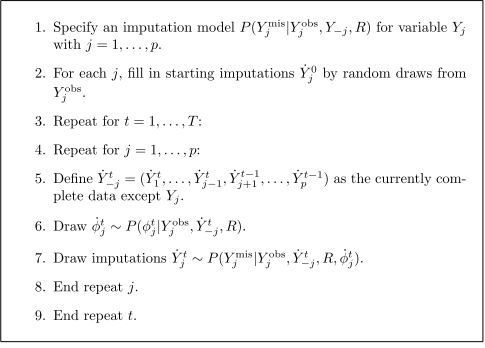
\includegraphics[width=0.8\textwidth]{fcs_algo}
  \caption{MICE FCS imputation pseudocode}
\label{fig:fcs}
\medskip
\small
Taken from van Buuren's book �Flexible imputation of missing data� \cite{VanBuuren2012}
\end{figure}

One of the major criticisms of this method is that in order for there to be a guarantee that we are sampling from the correct distribution, we need to ensure that our full conditionals are compatible, i.e. that they factor into the proper, explicit joint. This is very hard to check in practice, but multiple studies have shown that even when the models are highly incompatible, FCS methods are very robust and produce proper imputations \cite{VanBuuren2006}. FCS allows us much more flexibility than JM does, and it handles discrete and categorical data much better than JM does \cite{Kropko2014}. In addition, specifying the individual model for each covariate allows the user to handle the intricacies  of each covariate.

\begin{comment} Some popular R implementations of FCS methods include MICE \cite{VanBuuren2011}, mi \cite{Su2011}, and BaBooN \cite{Florian2015}, which go about drawing from the posteriors in different ways. These methods are good, but I will be using MICE in the applied section of this paper.
\end{comment}


The user is going to have to specify something, there is no escaping that, but it is easier for the average person to be able to define a single distribution and model rather than to guess at a multivariate distribution, particularly if it is high dimensional. In addition, in the survival analysis setting, there will naturally be strictly positive and categorical variables. Trying to fit a parametric distribution with these stipulations will be very hard if not impossible, so we will be relegated to using a general distribution (like the normal), which will certainly elicit a poor fit. So, JM approaches certainly seem ill-fitting, however FCS approaches are very appealing. 
\begin{comment}
In an ideal world, we would have complete data, and would not need to resort to imputation. But since we don't have complete data, we must choose one method and accept its strengths and weaknesses.
Might want to move elements of this down to application
Now that we have chosen the paradigm, we need to select an implementation of it. Many exist (such as MICE \cite{VanBuuren2011}, mi \cite{Su2011}, etc.). I wanted to select the implementation that combined ease of use, understanding, and programming. What I decided upon was a method called MICE- Multiple Imputation by chained equations \cite{VanBuuren2011} MICE is an FCS MCMC method that under compatibility, is a Gibbs sampler, where we obtain samples from the joint by sampling from the full conditionals. The user defines the full conditionals, so it is possible that the joint may only exist implicitly, and not actually have a functional form. 
\end{comment}

In order to use FCS methods properly, the missingness in our data must be MCAR or MAR. It can work with MNAR missingness, but it requires some extra modelling assumptions that are beyond the scope of this thesis. T tests have been proposed to test if the data is MAR or MCAR, but this is of little use for us, because we only want to know if the data is MNAR, which is impossible to test since testing for MNAR would entail us using information that is impossible to get \cite{Enders2010}. Luckily, we can safely assume MAR if there is reason to believe that some of the covariates collected account for the missingness \cite{VanBuuren2012}.


It should be noted that in the real data we will use, the response variable is fully observed, but the covariates have a lot of missingness. If it were the case that we had missingness in the survival time, then the methods described above might not work. They might fail because the unobserved times or outcomes may follow a different distribution than the observed times. This is cleared up by Zhao et. al in 2014 through Kaplan-Meier MI  \cite{Zhao2014}. This is beyond the scope of this report though so I omit its details. 

\subsection{Setting and checking the model}
Once we have established the MAR assumption, we need to set up our full conditionals imputation models. This may take a while for large datasets, but the extra time spent will ensure a better and move valid imputations. We choose what method to use (regression, predictive mean matching, logistic regression, trees, etc.), and then what predictors will go into those models. We should choose predictor variables that help explain missingness, as well as those we are doing inference on, as to avoid bias \cite{VanBuuren2012}. For variables that are derived from others, we impute its components and then compute that variable, in a process known as passive imputation. The full conditionals may also be parametric distributions if we so choose. With large datasets, we may need to perform variable selection before specifying the models, so that it doesn't become unmanageable.

Since FCS is an iterative process, we must choose how many iterations to do until convergence. The older literature suggests 5 iterations are enough, but with modern computation, we can easily exceed this, even with large data \cite{VanBuuren2012}. A good way to assess how many iterations to run is to look at the trace plots of the imputed values and then add 5 iterations to the number at which we assume convergence is achieved. Due to the nature of FCS methods, convergence is often very quick, often as soon as 5 iterations. As well, we need to decide how many datasets to impute. The early literature argued that 5 datasets would suffice, but modern literature argues for more, since it will cut down on simulation error. Many different authors have different criteria, but a popular criterion is to impute as many datasets as the 100 times the percentage of cases in the analysis with missingness. With the speed of computers and availability of storage, many authors now suggest using more imputations \cite{VanBuuren2012}.

Once we have determined how many iterations and imputations to run, the FCS algorithm is ran. Depending on the model specifications, it should not take too long for small datasets (seconds or minutes), but may take hours for larger ones. FCS models often converge quickly, so after convergence, we are just taking draws from the missing covariates posterior. The first few iterations may be considered as burn in, and the rest as samples. The value at the last iteration of each chain is taken as the sample from the posterior that will be used as the value for the missing data.

We need to verify that our imputations are valid once we complete them. First, we need to see if our chains have converged. Since FCS methods are  MCMC method, we should check the chains for irreducibility, aperiodicity, and recurrence. To determine when the chains have converged, van Buuren suggests that ``Convergence is diagnosed when the variance between different sequences is no larger than the variance within each individual sequence'' \cite{VanBuuren2012}.  There is some research (but not from the MI perspective) about tests to check for convergence, and a popular test is Gelman and Rubin's $\hat{R}$ scale reduction factor test \cite{Gelman1992}. This test is often used in conjunction with visual tests.  Assessing convergence  by looking at of all of the values over $m$ imputations and $k$ iterations would be very hard to visualize because there would be so many chains, so often times, we will choose to observe a statistic (like the mean) of the chain and assess on that. 

Once convergence is assessed, we need to check that the values imputed are valid and come from the correct posterior. This will serve as our model checking and validation. The overarching idea that we need to pay attention to is �does the data look like it could have been real data�. We can assess this in many ways, including density plots, box and whisker plots, scatterplots, histograms, etc. This is a visual task and there is no statistical method to validate this.

This whole process can be very time consuming because every time we want to make a change in the methods used, we have to rerun the algorithm and reassess our results. But once we find the setup that works for us, we don't need to repeat it again. So, while it may take a lot of time now, setting up a proper model will save us even more time in the future and ensure that our imputations are valid.

\subsection{Combining the MI estimates}
Once the $m$ datasets are imputed, we may run any valid analysis on each imputed dataset \textit{individually}, treating each of the $m$ datasets as if it was complete. Of course, the analysis in question should be run on the available cases, to ensure that the model assumptions are reasonable.

\begin{comment}
I am a strong advocate of running the model with the available cases if possible before running it on the MI data, so that we can assess the appropriateness of the model. As well, running the model with the available cases will give us a clue as to what to expect from the MI analyses (such as sign of the coefficients or level of significance).
\end{comment}


On the $m$ imputed data sets, we may then apply Rubin's rules \cite{Rubin1987} to pool our estimates. Rubin's rules are a set of rules that guide us in making inference from multiply imputed data. They will give us a single point estimate for the scientific estimand in mind, as well as the proper variance for it from the $m$ imputed datasets.  
%Do I need to make this bold?

Rubin's rules involve three parts. The first is getting an estimate of the population estimand $Q$, estimated with the MI datasets by $\bar{Q}$. To get $\bar{Q}$, define $\hat{Q}_i$ as the estimand evaluated from the data in the $i^{th}$ dataset.  Then, take the average over all $m$ datasets to get a single estimate $\bar{Q}$.
$$\bar{Q}=\frac{1}{m}\sum_{i=1}^{m}\hat{Q}_i$$
The estimates are not set, and there is variance associated with them. The first form of variance is the ``within'' variance, or the variance of each estimate $\hat{Q}_i$. This is the typical variance observed from having a sample. Define the variance covariance matrix of the $i^{th}$ imputed dataset as $\mathbf{\bar{U}_i}$ , then the overall within variance is computed as
$$\mathbf{\bar{U}}=\frac{1}{m}\sum_{i=1}^{m}\mathbf{\bar{U}_i}$$


The last form of the variance is the ``between datasets'' variance. This is the variance associated with the fact that we have missing data. It is given by
 $$\mathbf{B}=\frac{1}{m-1}\sum_{i=1}^{m}(\hat{Q}_i - \bar{Q})(\hat{Q}_i - \bar{Q})'$$

The total variance for our estimand is given by 
$$\mathbf{T=\bar{U}+B +\frac{B}{m}}$$
The last term is our simulation variance, and its existence is proven by Rubin in \cite{Rubin1987}.

The theory of inference with Rubin's rules is rooted in the assumption that under repeated sampling, the complete data quantity of interest is $Q-\hat{Q} $asymptotically normally distributed with mean 0 and variance $U$, where $U$ is the variance of $(Q-\hat{Q})$ \cite{VanBuuren2012}. We don't have the true population variance, so we must use what we have from the sample, namely $T$, the MI total variance. With this assumption, we know that
$$\frac{Q-\bar{Q}}{\sqrt{T}}\sim t_{\nu}$$ 
And the degrees of freedom is proven to be 
$$\nu=\frac{\nu_{old}\nu_{obs}}{\nu_{old}+\nu_{obs}}$$
Where $\nu_{obs}=\frac{\nu_{com}+1}{\nu_{com}+3}\nu_{com}(1-\frac{B + B/m}{T})$
, $\nu_{com}$ is the hypothetical complete sample degrees of freedom, and $\nu_{old}=\frac{m-1}{(\frac{B + B/m}{T})^2}$ \cite{Barnard1999}.

Rubin's rules assume normality, so if our statistic in mind is not asymptotically normally distributed, then we need to transform it towards normality before pooling. There have been some research about how to pool non normal quantities, but current research shows poor results and power when doing so \cite{Marshall2009}. We now have a powerful framework to get a single, valid estimate from multiply imputed data.

It should be noted that while Rubin's rules are the most popular method to combine MI estimates, there is another way to work with the multiply imputed data. This method is colloquially called the �stacked method�. For the stacked method, we take all of our imputed data and �stack� them one on top of each other to get one huge dataset of size $(m*i)$ rows and j columns. Under the stacked method, unbiased estimates of quantities of interest can be produced, but the estimates of variance will be too small (since we are artificially increasing the sample size) \cite{VanBuuren2012}. Thus, the stacked method is a poor choice for running any hypothesis tests or quantifying uncertainty. It is not useless though. The stacked method is useful when we want to analyze just one plot instead of $m$ for model checking. As well, the stacked method may be useful in situations where we partition categorical data on an imputed variable and then look at the percentage in each category. Under the averaging portion of Rubin's rules, we are not guaranteed that the percentages will sum to unity, but under the stacked method we are.


\section{Survival analysis}
\label{sec:Surv}
Now that we have the multiple imputation datasets created, we may run our analysis on each of them. Since the goal of this paper is cancer survival data, it naturally follows that the models we would like to run are survival models. As a general rule of thumb, we should run our desired analyses on the original available case data to get the available case estimates, as well as to get an idea of what to expect and to check if the model assumptions are met. Following Rubin's rules, we run the individual analyses on each of the $m$ datasets, and then pool our results. In this section we will discuss each type of survival analysis in the MI setting and the issues associated with them.

\subsection{Kaplan-Meier Survival Curve}
Analysis for the Kaplan-Meier estimate is quite simple in the non-MI setting, but special care should be taken in the MI setting. First, we need to clearly define what the groups and population are, and what constitutes an event of interest. A very common mistake that researchers make is to try to frame a competing risks problem as a Kaplan-Meier problem. We also need to be sure that we have non-informative censoring, that is, knowing that the individual is censored tells us nothing about their survival probability. Once we have checked all of these, we can compute the Kaplan-Meier curve on each of the $m$ datasets. For simplicity, in this section we assume that the Kaplan-Meier curves are run on a dataset with only subjects who take a treatment or a control. Now, we could pool these estimates, but that would be ill advised because the Kaplan-Meier curve is not normally distributed. To get around this, it has been proposed by Marshall et. al to take the complimentary log-log transformation of the survival estimates before pooling \cite{Marshall2009}. We can make this transformation, pool our results, and then back transform to get the pooled KM estimate. 

In the MI setting, an interesting situation may arise when the last event (and thus the range of survival time) differs between the imputed datasets. This is the result of a person with a long survival time being put in different groups via imputation. We can deal with this by either extending the last observed Kaplan-Meier estimate out until the last event time,  truncating all of the imputed curves at the minimum time of last event, or using other methods to deal with this situation as described in reference \cite{Klein1984}. In traditional analysis, we would not extend out the Kaplan-Meier curve out past the last event, but if we have wildly varying imputations, this might be a good option, so that we can make inference between curves and are not hampered by one poor imputed dataset. As well, we could use the stacked method to get the Kaplan-Meier estimates, but we must accept the fact that the variance at every time point will be too small.  The decision of what to do is up to the researcher and depends on the nature of the problem. 
\subsection{Median Survival Time}
One of the main tasks that clinicians are interested in is the median survival time of each group, which is the smallest time that the survival function for the group is less than 0.5. Since the true survival function is unknown, the Kaplan-Meier estimate is used. The median is the preferred method of central tendency in survival analysis because often times the survival times are right skewed, making the mean a poor estimator of the truth. Finding the median in the MI case is quite simple, as it is the first time that the MI averaged Kaplan-Meier curve crosses below 0.5. We would also like to have the variance at the median. The first way to obtain it is to multiply impute the variance (i.e. make the variance the scientific estimand of interest), and then use Rubin's rules to get the variance associated with each time point and then take the average as the variance at that time point. However, taking the mean and variance of the variance doesn't make much sense, and under typical pooling of the Kaplan-Meier estimate, we already get a good estimate of the variance. A better solution for this issue is to derive the variance of the median by the ``reflection method''. In this method, we first fit the MI Kaplan Meier curve, and then construct a 95\% confidence interval for all time points using the total variance obtained from Rubin's rules pooling. The median is defined as the first time when the pooled MI curve crosses 0.5, and the lower and upper 95\% confidence interval for the median are the medians of the upper and lower confidence bands. This method is preferred because it uses the variance we actually have and is much more robust to poor imputations.


\subsection{Log Rank Test}
Now we have a pooled estimate of the true survival curve for each group. In the typical setting, we might want to look to see if these curves are similar to each other, so we can determine if the treatment really prolongs survival time. We would do this with the log rank test under the regular setting. However, we should not be deceived. We have an MI averaged survival curve, which is not constructed in the same way that a regular Kaplan-Meier curve is, so we cannot get the quantities that we would need to compute the log rank test. However, we can still get the pooled log rank test. To do so, we can do one of two things. The first is to run the log rank test on each of the MI datasets and then pool the results via Rubin's rules. This is the logical way to do it, but under this scheme we will run into a multiple comparison problem. As well, Marshall shows that this method is unreliable and will not give the proper p-values \cite{Marshall2009}. Another option is to run a Cox regression on just the group in question, since this is equivalent to the log rank test under no tied failure times \cite{Klein1984}. Under tied failure times, they are very similar to each other. From the Cox regression, we can obtain the score test. We could pool the score test from each MI dataset, but we will once again run into problems. We could also try to run the score test on the pooled MI Cox regression model, however, in order to do this, we need to know who is in the risk set. But the concept of a risk set doesn't exist in the MI setting. Luckily, the Wald test is asymptotically equivalent to the score test, and the Wald test is very easy to obtain.  So we can use the Wald test of the coefficient from the Cox model as a proxy for the log rank test. In this way, we get a statistic that calculates what we want, while still making sense in the MI context.
\subsection{Cox Proportional Hazards Model}
We would now like to investigate the hazard ratio of different baseline covariates and treatments via the Cox proportional hazards model. The overall goal will be to fit a Cox model with baseline covariates, check to see if it passes the proportional hazards assumption, and then add in the treatment variables to see how they affect the hazard. It is known that the Cox regression coefficients are normally distributed, so there is no issue in pooling, but we do need to be careful about checking the proportional hazards assumption. The very first thing that we need to do is check to check the available case model to assess if we have proportional hazards. If one of the covariates truly is dependent on time, adding imputed data isn't going to change that, so checking the available case analysis is a good sanity check. The way we go about checking to make sure that we have proportional hazards is looking to see if the Schoenfeld residuals are uncorrelated with time for each covariate in the Cox model \cite{Schoenfeld1982}. The Schoenfeld residuals are tedious to explain and derive, and add no value to this thesis; however knowing that they are partial residuals that that are formulated to be independent of time should suffice to understand this paper.  The most common way to determine proportional hazards is to plot the spline fit (often cubic) to the residuals along with the 95\% confidence intervals, and see if any straight line could pass through the bounds. Because the residuals are independent of time, a straight line over time signifies that the hazards are proportional \cite{Schoenfeld1982}. There isn't an official name for this method, but the straight edge method seems to be a fitting name since you can check it by placing a straight edge between the confidence bands. If this is the case, then we say that that the covariate in question follows the proportional hazards assumption. Another method to check for proportional hazards is to use a chi square test of independence between the Schoenfeld residuals and time, although this is rarely used in practice.

If the proportional hazards assumption is not met, then we can add the variable that does not have proportional hazards into the model as a time dependent covariate. This is beyond the scope of this thesis, but is something that could certainly appear in practice.

We have discussed how to check the proportional hazards assumption in the available case scheme, but how can we do this in the MI setting? We can take our imputed data and fit a Cox model on each of the $m$ datasets, and pool them easily. But how is the best way to check the proportional hazards assumption? We can go about this in a few different ways. The first is to check the proportional hazards assumptions on each individual MI dataset. This may prove to be an arduous task especially with large $m$ and a large number of covariates in the model. Alternatively, we could superimpose all of the spline fits on one plot, and see how the shape and general trend compare to the available case analysis. We can also use the stack data to get just one set of plots, but the straight edge method will not work here since the errors are too low. 

Once we have verified that the model follows the proportional hazard assumption, we may trust its results. We can now add in our treatment covariates, and analyze it to see how they affect the hazards.

\section{Propensity Score Analysis}
\label{sec:Propscore}
Now that we have laid down the theory for analyzing the survival section for clinical relevance, we can move on to the causal analysis part. Viewing the analyses with a causal lens is important, because as of now with only survival analysis, we cannot be sure if the differences in treatments is actually due to the treatment or to some pretreatment group differences. While there is a lot of preparatory work that goes into the theory of it, the results that can be obtained using causal analysis framework and propensity scores is much stronger and appealing than conventional analysis.  Although no statistical method will give us a causal relation, the results from causal analysis will be much more similar to the results we would have got from a RCT.

Propensity score methods are an easy to understand yet powerful tool to help implement Rubin's causal model. The use of propensity scores justified in Rosenbaum and Rubin's 1983 paper \cite{Rosenbaum1983}.  Our overall goal is to estimate the average treatment effect in a setting where the initial study was not an RCT. We will use the propensity scores to balance the groups and remove the effect of confounders, so that the data seems more like an RCT. 

Before we even begin using propensity scores, we should have in mind what estimand we wish to estimate (the ATE or the ATT). It should be noted that while the ATE and ATT deal with means, the definition can be modified so that it can deal with the difference in hazard ratios \cite{Austin2014}. The choice of estimands should be done by addressing the problem and discussing the implications of each with subject matter experts. Once we have this, we can start out with the propensity score methods. 

\subsection{Selecting the method}
We will need to make many decisions along the way, both in how to use the propensity scores, and how to combine them with the MI data. There are four main uses of propensity score in the literature: matching, stratification, weighting, and covariate adjustment \cite{Austin2014}. The goal is to balance the treatment and control groups, such that the only difference between the groups is due to the treatment received, and not any underlying factor. All of these methods will help us to examine the average treatment effect, but each goes about it in a different way. Covariate adjustment and matching have fallen out of favor in the literature recently, but weighting and stratification remain very popular \cite{ Austin2014}. We will be using weighting in our real data analysis, so the main focus will be on that, but the methods discussed will work with any propensity score method. Whatever method is chosen will need to be run on the MI datasets. The stacking method described before would obviously be inappropriate, as the sample size will be too large, and with high probability, subjects will be matched to themselves. Thus, the analysis will not be valid 

Since the stacking method will not work, we must decide how to use propensity scores on the multiply imputed data. Two methods are described in Mitra and Reiter about how use propensity scores in the MI setting \cite{Mitra2012}. In both methods, the propensity scores are first computed for each MI dataset, as we would normally do in the analysis part of the MI process. However, how the two methods use the propensity scores are different. In the first method, known as the ``within '' method, the propensity score method is done within each MI dataset and then pooled. For example, if we wanted to find the ATE, we would estimate the ATE in each dataset, and then pool via Rubin's rules. The other method, known as the ``across'' method, takes the $m$ estimates of each individuals propensity scores between the MI datasets, and then averages them so that every subject has one averaged propensity score. Once the global averaged propensity scores are estimated, then the propensity score method is used in each dataset (using the global list), the ATE is estimated on each dataset, and then pooled via Rubin's rules. Both methods have their pros and cons, and are appropriate for different scenarios. 

\begin{comment}
However, the treatment variable may itself have missingness, and thus needs to be imputed. In this situation averaging across datasets does not make sense (since there is no guarantee that a given subject in imputation $i$ has the same treatment in imputation $j$), so we cannot determine if the subject is a case of a control, thus matching will be impossible. When this is the case, we must use the within method. 

\end{comment}
%does the fact that the drug is an imputed value effect which model we should use? The problem exists %that the treatment is unknown in some, so it needs to be imputed.  Thus, we could have 30 datasets %where subject I is treatment, and 20 where he is a control. We can either classify as treatment via %majority voting. If not this, then we need to change to the within method.
\subsection{Obtaining the Propensity Score}
Now that we have discussed the method about how to use propensity score methods in the MI setting, let's discuss how to actually get the propensity scores for each MI dataset. From now on, propensity score weighting will be the only method discussed, because that is what will be used in the application section.

Different propensity scores will be obtained according to what pretreatment covariates we use in the propensity score model, so we need to be sure that model is fit with clinically relevant and meaningful predictors. Recall that our overarching goal is to account for any pretreatment covariate that confounds the selection of the treatment, and to try to make the no unmeasured confounders assumption more reasonable. There has been significant debate among statisticians about how to set up these models, by either throwing in every possible variable into it, or only include covariates known to affect treatment selection. I don't plan to settle this debate, but I do believe that the user should account for everything that is believed to be different between the two groups in question, in order to make the no unmeasured confounders assumption more plausible. 

Obtaining the propensity scoring using logistic regression is simple and has been historically used, but with newer machine learning methods, we are able to get better propensity score weights that induce more balance (which will be talked about next). For single analysis, logistic regression would be preferred due to its simplicity and power, but in the MI setting, the model that fits well for one dataset might not fit well for another one. That is why machine learning methods are preferred. In recent years, boosting has become very popular method to compute propensity score weights, because they can be selected in a way to achieve optimal balance\cite{McCaffrey2013}.

\subsection{Verifying Balance}

The goal of weighting is to create a pseudo-sample that is balanced, by up weighting samples that look like treatment cases, and down weighting those who do not. The formula for each weight can be concisely given as $w_i=\frac{T_i}{\hat{e}_i(x)}+\frac{1-T_i}{(1-\hat{e}_i(x))}$, recalling that T is the treatment indicator, so only one of these terms is ever not 0. Two methods have been suggested to check for balance. The first is known as standardized bias. For each pretreatment covariate we wish to balance, we see how similar the cases and controls are by observing $|\bar{X}_{k1}-\bar{X}_{k0}|/ \hat{\sigma}_k$, where the barred X's denote the weighted means of the covariate in the treatment and control groups, and the $\hat{\sigma}$ is the unweighted standard deviation of both groups together. Typically, standardized bias below .2 or .25 indicates good balance, although this number is subjective. Another common method is the Kolmogorov�Smirnov (KS) test of distributional equality. In this nonparametric test, the Empirical Cumulative Distribution Function (ECDF) is computed for the two (weighted) groups. Then, the maximum distance between the two ECDF's is calculated. Its p-value is found via the permutation test for the null hypothesis of no differences in the distribution \cite{McCaffrey2013}.


Both of these methods offer us tools to assess balance in the data when weighted by the propensity scores. We can use the tools to our advantage alongside of a boosting algorithm to get good balance. In boosting, a simple piecewise linear function is fit to the data, and after every iteration, a new piecewise linear function is fit to the previous models residuals. We can boost our data, weight each observation by its propensity score, and then check the balance at each iteration of the boosting algorithm. The goal is to find the propensity score weights that minimize either the standardized bias or the KS statistic, although minimization of one often leads to significantly better balance in the other metric.

Once we have obtained our optimal propensity scores for each MI dataset, we weight the data by them. Then, we check to see if we have balance. As well as checking that we truly have achieved balance, we also need to look at the distribution of the propensity scores. We would like to see some overlap between the treatment and control propensity scores. Overlap indicates that subjects in both groups are similar to each other, and can be compared. If the propensity scores don't have any common support, then we have not properly balanced. We should also be sure that all of the propensity scores are bound between zero and one. If a subject has a propensity score that is either one or zero, then they will always be or never be treated, and estimating the counterfactual will be ill-advised.

Once we have our propensity scores, we need to go about checking the treatment effect. We have no guarantee that the model we set for our propensity score is correct, so many authors advocate including troublesome variables in the analysis of the treatment effect (this is known as a doubly robust method) \cite{Lunceford2004}. 

Now that the theory is set up, we may use it on the MI data. And now we may interpret the results with a causal lens, even though the data may be observational. We will be using the within method, so for each MI dataset, we compute the treatment effect from the propensity score weighted data. While we could check the treatment effect in terms of time difference in survival between the treatments, this doesn't work very well, because we have censored data. The better option is to observe the average treatment effect by looking at the change in the hazard between the treatment groups. Checking the hazard makes use of the fact that we have censoring in the data. We may then combine the estimates via Rubin's rules to get the MI estimate of the average treatment effect and its variance.
\begin{comment}
The matching can be done in many different ways like a nearest neighbor, caliper, or mahalanobis distance matching. It shouldn't really matter which one we use, so long as the groups are similar in distribution after matching in each dataset.
Once an acceptable propensity score model is selected, we will need to pick what type of weighting we will do. Many exist, but the most popular are X,Y,Z . We will then run our Cox model again (as in the survival section), but we will factor in the weights. Then, the results that we receive can be viewed as if they were from a RCT. As well, we can go ahead and analyze them as such, and draw causal inference. I need a lot more work here.

\end{comment}


